\documentclass{beamer}

\usetheme{CambridgeUS}
%\usecolortheme{albatross}

\usepackage{graphicx} 
\usepackage{booktabs} 

\title[Week 2 Review]{EPSRC Vacation Scheme: Mid-Project Review} 

\author{Matthew Knowles} 
\institute[UoY] 
{
Department of Mathematics \\
University of York \\ 
\medskip
\textit{mk1320@york.ac.uk} 
}
\date{$31^{st}$ August 2021} 

\begin{document}

\begin{frame}
\titlepage 
\end{frame}

\begin{frame}
\frametitle{Goals}
\begin{enumerate}
	\item Implement Convex Hull Approximation 
	\pause
	\item Look into making it more efficient

\end{enumerate}
\end{frame}

\begin{frame}
\frametitle{Task 1 Progress}
\begin{itemize}
	\item This was so much more difficult than I had expected
	\pause
	\item Arguably spent too long worrying about something not entirely related  
	\pause
	\item Switched from Thesis to paper as to not worry too much about generalisation
\end{itemize}
\end{frame}


\begin{frame}
    \frametitle{Fixing the discontinuity}
        \begin{figure}
            \center
            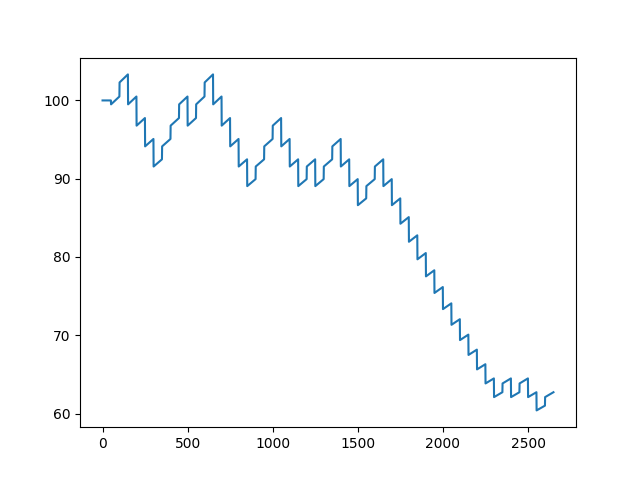
\includegraphics[scale=0.6]{../Figures/upperapproxattempt2.png}
        \end{figure}
\end{frame}

\begin{frame}
\frametitle{Issues}
\begin{itemize}
	\item Well it's not convex for a start
	\pause
	\item Also not really a hull
	\pause
    \item Hope is not lost: Enter RouxHull!
\end{itemize}
\end{frame}

\begin{frame}
    \frametitle{Random Walk}
        \begin{figure}
            \center
            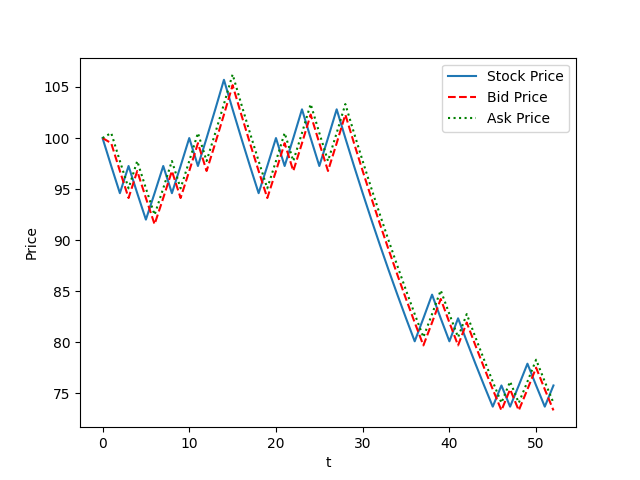
\includegraphics[scale=0.6]{../Figures/upperapproxstockprice.png}
        \end{figure}
\end{frame}

\begin{frame}
    \frametitle{Next steps!}
    \begin{itemize}
        \item The above graph is taken from: $$ S_{t+1} = 
        \begin{cases}
            e^{\sigma\sqrt{\frac{1}{52}}S_t}, & p \\
            e^{-\sigma\sqrt{\frac{1}{52}}S_t}, & 1-p
        \end{cases}
        $$ (Roux, 2021)
        
        \item Calculate bid and ask prices via $S_t^a = (1+k)S_t$, $S_t^b = (1-k)S_t$
        \item Create $n-1$ subintervals for each $t=0,\ldots,T-1$ via: 
        $$
            s^i_t = S^b_t + \frac{i-1}{n-1}\left(S^a_t-S^b_t\right)
        $$ for $i = 1,\ldots,n$
    \end{itemize}
\end{frame}
\begin{frame}
    \frametitle{Next steps! (contd)}
    \begin{itemize}
        \item Now implemetnt (A.10) from 2021 paper$$
        \hat{f_k}(x) = 
        \begin{cases}
            f(\hat{x}_{kl}) & \text{if } x=\hat{x}_{kl} \\
            \frac{\hat{x}_{kl}-x}{\hat{x}_{kl}-\hat{x}_{k[l-1]}}\hat{f_k}(\hat{x}_{k[l-1]}) + \frac{x-\hat{x}_{k[l-1]}}{\hat{x}_{kl}-\hat{x}_{k[l-1]}}\hat{f_k}(\hat{x}_{kl}) & \text{if } x \in (\hat{x}_{[l-1]},\hat{x}_l)\\
            \infty & \text{if } x \notin [b,a]
        \end{cases}
        $$
        \item With this, apply RouxHull to get the upper approximation
    \end{itemize}
\end{frame}

\begin{frame}
    \frametitle{A hull!}
    \begin{figure}
        \center
        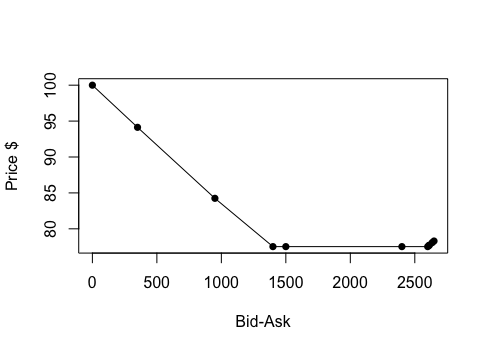
\includegraphics[scale=0.6]{../Figures/finalexamplehull.png}
    \end{figure}
\end{frame}

\begin{frame}
    \frametitle{Work to be done}
    \begin{itemize}
        \item Putting hull onto bid-ask graph (Pyhton issue)
        \pause
        \item Looking for ways to optimise
        \pause
        \item Genetic Algorithms??
    \end{itemize}
\end{frame}

\begin{frame}
    \frametitle{Some bloopers}
    \begin{figure}
        \center
        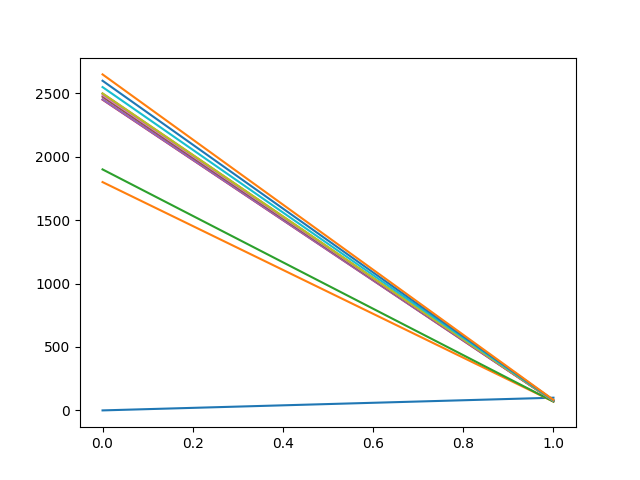
\includegraphics[scale=0.6]{../Figures/hullblooper.png}
    \end{figure}
\end{frame}

\begin{frame}
    \frametitle{I have no idea how to explain this}
        \begin{figure}
            \center
            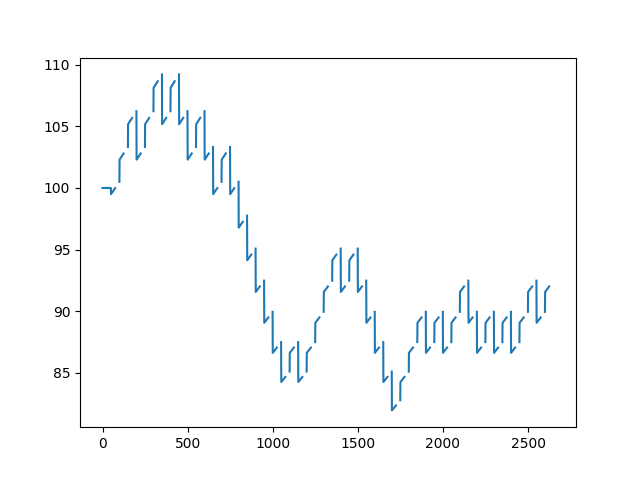
\includegraphics[scale=0.6]{../Figures/whatonearth.png}
        \end{figure}
    \end{frame}

\end{document} 